%% The first command in your LaTeX source must be the \documentclass command.
%%
%% Options:
%% twocolumn : Two column layout.
%% hf: enable header and footer.
\documentclass[
twocolumn,
% hf,
]{ceurart}

\usepackage{algorithm}
\usepackage{algpseudocode}
\usepackage{hyperref}

%\usepackage{svg}
\usepackage{multirow}
\usepackage{caption}
\usepackage{tikz}
\usepackage{amssymb}

%\usepackage[semicolon]{natbib}

%%
%% One can fix some overfulls
\sloppy

%%
%% Minted listings support 
%% Need pygment <http://pygments.org/> <http://pypi.python.org/pypi/Pygments>
\usepackage{listings}
%% auto break lines
\lstset{breaklines=true}

%%
%% end of the preamble, start of the body of the document source.
\begin{document}

%%
%% Rights management information.
%% CC-BY is default license.
\copyrightyear{2025}
\copyrightclause{Copyright for this paper by its authors.
  Use permitted under Creative Commons License Attribution 4.0
  International (CC BY 4.0).}

%%
%% This command is for the conference information
%\conference{EXAG 2024: AIIDE Workshop on Experimental AI in Games, November 18--22, 2024, Lexington, KY, USA}
\conference{ }


\title{ A Generalized 2D and 3D Hilbert Curve }

\author{Jakub \v{C}erven\'{y}}[url=https://github.com/jakubcerveny]
\author{Zzyv Zzyzek}[url=https://zzyzek.github.io,orcid=0009-0005-2175-1166]



\begin{abstract}
The two and three dimensional Hilbert curves are fractal space filling curves that
map the unit interval to the unit square or unit cube.
Hilbert curves preserve locality, keeping distance from the unit interval
to their respective higher dimensional embeddings.
Finite approximations of the Hilbert curve can be constructed in stages
by stopping the recursive construction at a specified depth, providing locality
from a discrete array of points to points in the embedded dimension.
The locality property of the Hilbert curve can help with caching optimizations based on order
and finds uses as a companion method in applications ranging from job scheduling
to scene rendering.
One limitation of the Hilbert curve approximation construction is that the regions need
to be exact powers of two, making it difficult to work with in many real world
scenarios.
In this paper, we present the Gilbert curve,
a conceptually straight forward generalization of the Hilbert curve,
that works on arbitrary rectangular regions.
The construction provides reasonable worst case run-time guarantees for random
access lookups for both two and three dimensions.
We also provide comparisons to other Hilbert curve generalization methods
and investigate overall quality metrics of the Gilbert curve construction.
\end{abstract}

\maketitle

\newcommand{\specialcell}[2][c]{\begin{tabular}[#1]{@{}l@{}}#2\end{tabular}}
\newcommand{\specialcellCenter}[2][c]{\begin{tabular}[#1]{@{}c@{}}#2\end{tabular}}

\section{Introduction}

\subsection{Overview}

We present the \textit{Gilbert curve}, a generalized Hilbert curve for 2D and 3D,
that works on arbitrary rectangular regions.
%We call our realization of the generalized Hilbert curve a \textit{Gilbert curve}.

An overview of the benefits of the Gilbert curve are that it is:

\begin{itemize}
  \item Valid on arbitrary rectangular regions
  \item Efficient at random access lookups ($O(\lg N)$)
  \item A conceptually straight forward algorithm
  \item Able to realize curves without notches unnecessarily and limits the resulting curve
        to a single notch when forced
\end{itemize}

Further, we show:

\begin{itemize}
  \item Equivalent to the Hilbert curve when dimensions are exact powers of 2
  \item Measures of locality are preserved (Section X)
  \item Comparison metrics to other space filling curves (Section X)
\end{itemize}

Some drawbacks are that:

\begin{itemize}
  \item Our implementation is recursive,
        which may be undesirable for some applications requiring better than $O( \lg N)$
        memory usage or better constant bounds for runtime performance
  \item Might not adequately capture some features of a Hilbert curve
\end{itemize}


Generalizations of the Hilbert curve to non power of two rectangular cuboid regions
have been explored before but are overly complicated algorithmically, create unbalanced
curves and often don't generalize well to 3D.
Our realization focuses on a conceptually simple algorithm which creates pleasing
resulting curves and works in both 2D and 3D.

Space filling curves are a specialization of a more general Hamiltonian path,
but have a more stringent requirement of local connectivity.
The local connectivity, or locality, preserves a measure of nearness, where
points from the source unit line remain close in the embedded space.

% this section might be unncecessary
%
%The local connectivity requirements
%preclude things like \textit{zig-zag} Hamiltonian
%paths, paths that run straight from one side to another before turning around,
%as nearby points in the embedded dimension can be far from the origin line.

% FIGURE DESCRIBING LOCALITY, LOCAL CONNECTIVITY


The Gilbert curve algorithm works by choosing sub rectangular cuboid regions
to recursively find a connecting path.
If one extent of the cuboid becomes too large or small relative to the other lengths,
a special subdivision is performed to try and make further subdivisions more cube-like.
Subdivisions are performed until a base case is reached and the lowest unit of the curve
can be realized.

A Hamiltonian path is not always realizable for certain side lengths and endpoint constraints.
In such a case, the Gilbert curve will introduce a single diagonal path move, called a \textit{notch}.


\subsection{Definitions}

A Gilbert curve is %, for a rectangular cuboid region, is
%To describe the Gilbert curve algorithm, we concern ourselves with
%finding
a self avoiding path,
restricted to the cubic lattice graph in a rectangular region, that also has locality.
That is, we want to find a Hamiltonian path, with pre-specified start and end points, that hit
every vertex within a cuboid rectangular region exactly once with any points close on the curve
being appropriately close in the cubic lattice.

Here, the \textit{cubic lattice graph} is a graph
whose vertices are the integral points in $\mathbb{Z}^3$, with edges joined between them when they
are unit distance away.

A discrete \textit{path} is an array of points, $\omega = (\omega_0, \omega_1, \dots, \omega_{N-1})$, where each $w_i$ is on the
cubic lattice graph ($w_i \in \mathbb{Z}^3$).
A \textit{self avoiding path} $\omega$, is one that does not visit a previously vertex ($i \ne j \to \omega_i \ne \omega_j$).
A \textit{Hamiltonian path} is a valid path through a graph that visits every vertex exactly once, starting
and ending at pre-specified points.

A \textit{cuboid} is a rectangular region of side lengths $( N _ x, N _ y, N _ z)$,  of total vertices $N = (N _ x \cdot N _ y \cdot N _ z)$.
A cuboid region is said to have a \textit{feasible} Hamiltonian path if there exists a Hamiltonian path, with endpoints specified,
that hits every vertex within the cuboid region exactly once, starts at the specified start
point, $\omega_0$ and ends at the specified endpoint $\omega_{N-1}$.
A cuboid region that cannot have a Hamiltonian path, with the specified endpoints, is said to be \textit{infeasible}.

A self avoiding path of length $N$ that is confined to the rectangular region $(N_x, N_y, N_z)$ is necessarily a Hamiltonian path.

A discrete realization of the Hilbert curve as a path within a cuboid region has an additional \textit{local connectivity} feature.
For our purposes, \textit{local connectivity}, or \textit{locality}, denotes the idea that if $\text{dist}_1(i,j)$ is small, then $\text{dist}_d(w_i,w_j)$
should also be small by some measure, where $\text{dist}_d(\cdot,\cdot)$ is a distance function defined for dimension $d$.
The condition of a Hamiltonian path through a cuboid region doesn't address locality and the Gilbert curve
has additional features to make its locality similar to the Hilbert curve.
%We only provide some intuitive explanation for local connectivity here.
%That is, nearness in the line domain should relate to nearness in the three dimensional range.
We use metrics to get a handle on local connectivity in a discrete and finite setting and leave
their definition and usage until Section 5.


%A consequence of the Hahn-Mazurkiewicz \cite{sagan_1994} one can map the unit interval on the real line to a three dimensional
%cube if and only if the mapped to space is compact, connected and locally connected.
%We concern ourselves with the concept of \textit{local connectivity} with attention to approximations
%to finite realizations of curves on the 2D and 3D lattice.

%% sectoin might be too extraneous
The concept of local connectivity gives one of the key characteristics of a space filling curve
and differentiates it from other curves that can fill rectangular regions but don't do so in a
locally connected way \footnote{For example, the \textit{zig-zag} curve that creates a straight line until
it hits the bounds of the region to turn around and increment in the other dimensional lengths to fill 
a rectangular region.}.
The local connectivity, or locality, is the feature that allows clustering in dimension one to
remain clustered in higher dimensions \footnote{We refer the reader to
Sagan \cite{sagan_1994} for a more thorough introduction to local connectivity.}.

If a cuboid region has one side larger or smaller than the maximum or minimum of the remaining two, respectively,
for a given ratio, $\rho$, it is said to be \textit{eccentric}. % or $\rho-\textit{eccentric}$.
For example is, if $\rho=\frac{3}{2}$ and $N _ x > \frac{3}{2} \text{max}(N_y, N_z)$, the cuboid region is said to be eccentric.

In this paper, we talk about \textit{shape templates} as cuboid subdivision schemes, often with some choice as to whether
to make the side lengths of the subdivided regions even or odd.
For 2D, we use the term $U$-split to talk about the shape template used.
For 3D, we use the term $J$-split to talk about the bulk recursion shape template and an $S$-split to
talk about the shape templates used for eccentric cuboids.

%For simplicity, we focus on three dimensions with the understanding that
%the two dimensional case can be reduced to a three dimensional case with at least one unit side length.

\section{Related Work}

Peano discovered the first space filling curve, with Hilbert later discovering
a space filling curve that we concern ourselves with in this paper \cite{hilbert2004david}.
Hilbert's curve takes a one dimensional line and maps it to a compact, connected and locally connected
set.
For an introduction to space filling curves in addition to the necessary and sufficient
conditions for a space filling curve, the reader is referred to Sagan \cite{sagan_1994}.

As an artifact of the construction scheme, the Hilbert curve requires the side lengths to be exact powers of two.


%---
%
%Rong, Zhang and Lin provide a modified Hilbert curve to arbitrary rectangular cuboid regions,
%with an application towards image and video compression.
%  - subdivide by lopping off largest power of two
%  - can lead to long straight edges in normal conditions (7a) (?)
%  - non-unique
%  - complicated (?)
%  - only works on $W \times H \times 2^d$ (?!)
%
%Zhang, Kamata, Ueshige, "pseudo-Hilbert scan for arbitrary-sized arrays"
%  - 2d (only)
%  - complicated (?)
%  - doesn't generalize well to 3d (?)
%  - aeshetically not so nice (see fig 7c, 7d)  (?)
%
%Voorhies coherence measure (graphics gems) seems pretty simple and reasoable?
%
%Dafner, Cohen-Or and Matias use a \textit{context-based} space filling curve that
%uses an underlying image to ...????
%
%Lianyin etal. propose more efficient encoding and decoding algorithms for 3d Hilbert
%curves ...
%
%Haverkort enumerates unique 3d Hilbert curves ... but doesn't require subdivided
%cubes to be next to each other, so potentially has large skips/diagonal moves from
%one to another?
%
%Haverkort also creates an 'inventory' of 3d Hilbert curves that "share the same properties"
%as 2d Hilbert curves.
%  - looks to be restricted to powers of 2
%  - vertex continuous (which is what we want)
%  - has many definitions of locality and others that might be interesting
%
%Haverkort and Walderveen define some "locality and bounding box quality" metrics,
%presumably to measure sfcs
%
%Haverkort 'recursive tilings .. little frag' introduces Arrwwid numbers
%
%
%B{\"o}hm, Perdacher and Plant propose Hilbert traversal order for problems
%such as K-means, Cholesky decomposition and matrix multiplication so as to exploit
%better cache utilization from the the locality of the Hilbert curve.
%
%Gotsman and Lindenbaum quantify locality and show Hilbert curves are optimal in relation
%to their metric.
%
%Mokbel, Aref, Kamel define \textit{Jump, Contiguity, Reverse, Forward and Still}.
%Incorrectly call scan and sweep curves/paths space filling.
%
%

\section{Algorithm}

\subsection{Overview}

We discuss one possible generalization of the Hilbert curve, which we call the Gilbert curve,
to arbitrary axis-aligned cuboid regions.

The design of the Gilbert curve is done to provide a:

\begin{itemize}
  \item Conceptually simple algorithm
  \item Harmonious realization
  \item Resulting curve with good locality conditions
\end{itemize}

The discretized Hilbert curve recursively traces out a Hamiltonian path through a square
region whose sides are powers of two.
The Gilbert curve extends this idea to trace out Hamiltonian paths through to arbitrary axis-aligned
cuboid regions.

The Gilbert curve recursively subdivides a larger cuboid region into smaller cuboid
regions of different sizes and orientations.
The subdivision scheme uses a shape template that will be explained in more detail in subsequent sections.
The orientations of the subdivided cuboid regions are chosen so that the recursive path
will start and end at pre-specified endpoints, connecting neighboring cuboid regions
after a path is realized.

If a cuboid becomes too oblong, or \textit{eccentric}, a subdivision shape template scheme is chosen
in an attempt to create subdivisions that are closer to being cube like.

%The cuboid region is represented by an origion point, $p \in \mathbb{Z}^3$,
%and a local coordinate system of three vectors $\alpha, \beta, \gamma \in \mathbb{Z}^3$.

The subdivided cuboid region is processed by the Gilbert curve algorithm,
with virtual origin point $p \in \mathbb{Z}^3$ and local coordinate system $[ \alpha, \beta, \gamma ]$,
with $\alpha, \beta, \gamma \in \mathbb{Z}^3$.
Each of $\alpha$, $\beta$ and $\gamma$ are axis aligned and orthogonal.

In a cuboid region, the the Hamiltonian path start at $p$ and ends at $p + \alpha$.
For this reason, we call $\alpha$ the ``width-like'' dimension, with $\beta$ and $\gamma$
called the ``height-like'' dimension and ``depth-like'' dimension, respectively.

When processing the subdivided cuboid regions, the coordinate system is updated
with new integral lengths and rotated.
Since rotations are only in units of $(\pi/2)$ radians and $\alpha$, $\beta$, $\gamma$ start
off as axis-aligned and orthogonal, they remain axis aligned and orthogonal throughout.

%Using parity arguments, the possibility of a Hamiltonian path it's not difficult to show that
%if a Hamiltonian path is possible or not.
%for a given side lengths along with a start and end point,
%combined with certain cuboid side lengths,
When applying the shape template to choose the subdivided cuboid regions during the coarse of the
algorithm, side lengths are chosen so as to preserve the possibility of a Hamiltonian path.
Should the lengths of the cuboid being subdivided preclude a Hamiltonian path from occurring, the lengths
of the subdivided cuboids are chosen
so that all but one will preserve the possibility of a Hamiltonian path.
In this case, since only a single cuboid absorbs the impossibility of a Hamiltonian path,
and this process is recursively applied, there will be a single jump, or \textit{notch},
in the resulting curve, globally.

%Each of $\alpha$, $\beta$ and $\gamma$ start off as axis-aligned vectors of integral
%length and are only rotated by units of $(\pi/2)$ radians, remaining axis aligned throughout.
%$\alpha$, $\beta$ and $\gamma$ represent the dimensions of the sub-cuboid region
%and the local basis when tracing out a curve.

The next sub-section discusses parity arguments for when a valid curve can be
traced out in a sub-region.
We then discuss in detailed the 2D Gilbert curve algorithm and end with a discussion of the 3D Gilbert curve.

When talking about the 2D Gilbert curves, we assume vectors are in $\mathbb{Z}^3$
so they can be used without alteration for algorithms working in 3D.

%In what follows, a path is assumed to start at the local reference point $(0,0,0)$
%and end at the far edge of the the width like dimension, $\alpha$ (e.g. $(w-1,0,0)$).

\subsection{Valid Paths from Grid Parity}

\begin{figure}[h]
  \centering
  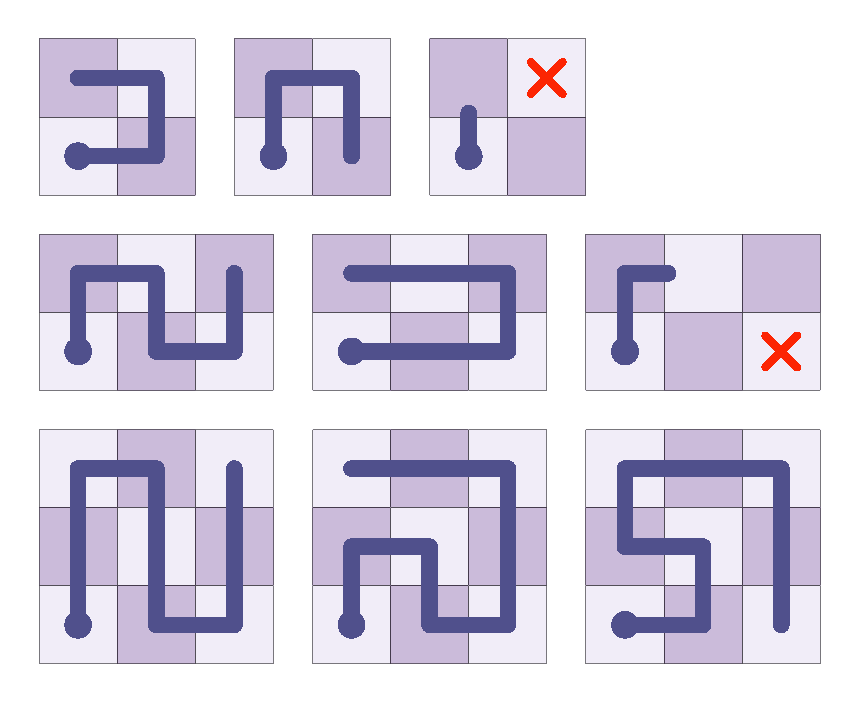
\includegraphics[width=\linewidth]{simple_hampath.pdf}
  \caption{ Illustrative examples of Hamiltonian paths height/width that are even/even, even/odd and odd/odd, respectively,
            when starting from the lower left hand corner }
  \label{fig:exampleHampath}
\end{figure}


The feasibility of determining whether there exists a Hamiltonian path in a rectangular cuboid
grid region can be accomplished through parity arguments.
Label grid cell points in a volume as 0 or 1,
alternating between labels with every axis-aligned single step move.
Any Hamiltonian path that ends at one of the three remaining corners has to have the same parity as the starting point if the
volume is odd, or different parity if the volume is even.

\begin{table}[h]
  \centering
  \begin{tabular}[t]{cr|cc}
    \multicolumn{2}{c}{ \multirow{2}{*}{Path Possible} } & \multicolumn{2}{c}{Volume} \\
    & & \textit{even} & \textit{odd} \\
    \hline
			%\multirow{2}{*}{$|\alpha| \bmod 2$} & \textit{even} & Yes & Yes \\
      \multirow{2}{*}{ $|\alpha|$ } & \textit{even} & Yes & Yes \\
       & \textit{odd} & \textbf{No} & Yes \\
     \hline
  \end{tabular}
  \caption{ Table showing when a Hamiltonian path is possible. Here, $|\alpha|$ is the absolute difference in start and end position of the path which
            coincides with one of the axis aligned side length of the cuboid volume. A Hamiltonian path is not possible on only in the case
            when $|\alpha|$ is odd and the volume is even. }
  \label{table:pathTable}
\end{table}


For a path starting at $(0,0,0)$ and ending $|\alpha|$ steps in one of the axis-aligned dimensions,
then Table \ref{table:pathTable} enumerates this condition under which a valid path is possible.
Figure \ref{fig:exampleHampath} illustrates this for starting position $(0,0)$ with volumes $(2 \times 2)$, $(3 \times 2)$ and $(3 \times 3)$,
where a red cross indicating a precluded endpoint.

Without loss of generality, we will assume a curve starts from position $p_s=(0,0,0)$ and has proposed
endpoint at $p_e=((w-1),0,0)$, with a cuboid region as $\alpha = (w,0,0), \beta = (0,h,0), \gamma = (0,0,d)$.
We state, without proof, that
a Hamiltonian path is always possible from $p_s$ to $p_e$ when $|\alpha|$ is even or when $|\alpha|$, $|\beta|$ and $|\gamma|$
are all odd  $(|\alpha| \cdot (1 - |\beta| \cdot |\gamma|) \equiv 0 \bmod 2)$.

With this condition, any cuboid subdivision will always have a Hamiltonian path within it and we can recreate a Hamiltonian
path in the larger cuboid by connecting endpoints from the ending point of one cuboid to the starting point of the succeeding cuboid.
For cuboids that violate this condition, there will be a required notch and
an admissible cuboid subdivision is possible
for all but one of the cuboid subdivisions, recursively limiting the notch violation to a single point.


%%%%%%%%%%%%%%%%%%%%%%%%%%%%%%%%%%%%%%%%%%%%%%%%
%            _ ____              __ ___       __
%     ____ _(_) / /_  ___  _____/ /|__ \ ____/ /
%    / __ `/ / / __ \/ _ \/ ___/ __/_/ // __  / 
%   / /_/ / / / /_/ /  __/ /  / /_/ __// /_/ /  
%   \__, /_/_/_.___/\___/_/   \__/____/\__,_/   
%  /____/                                       
%%%%%%%%%%%%%%%%%%%%%%%%%%%%%%%%%%%%%%%%%%%%%%%%


\subsection{2D Generalized Hilbert Function (Gilbert2D)}

\begin{figure}[h]
  \centering
  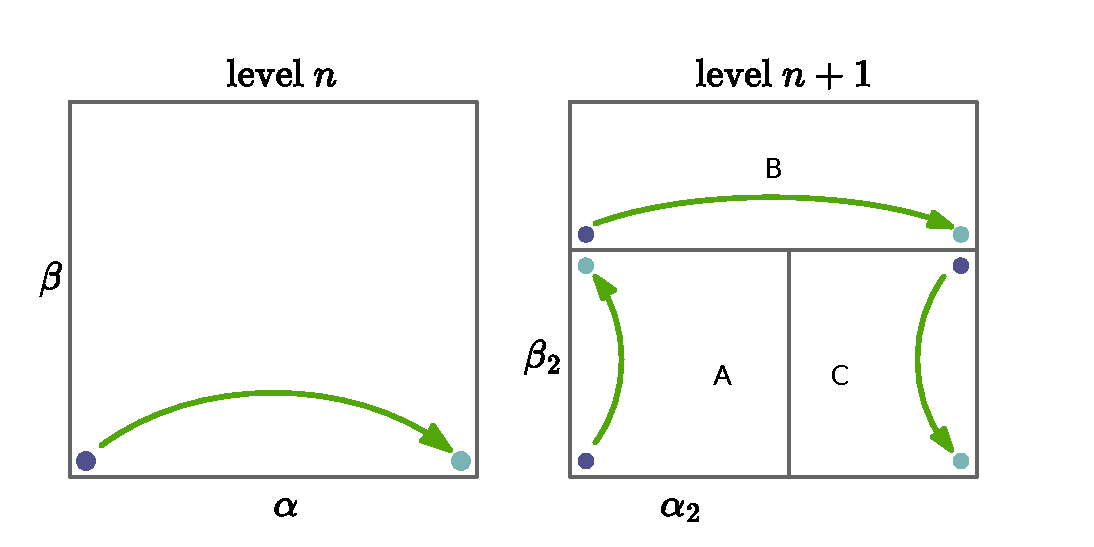
\includegraphics[width=\linewidth]{gilbert2d_mainsubdiv.pdf}
  \caption{ For the 2D Gilbert curve, the main rectangle is subdivided into three sub regions, making sure their paths connect
            and preferring even side lengths for the first rectangular subdivision.
            Partitioning the rectangle in this way is what we call a $U$-split.  }
  \label{fig:main2dsubdiv}
\end{figure}


\begin{figure*}[ht]
  \centering
  \includegraphics[width=\linewidth]{config_production.pdf}
  \caption{ Enumeration of the subdivision template depending on different parities of $\alpha$ and $\beta$ dimensions. }
  \label{fig:production2d}
\end{figure*}

For the 2D Gilbert curve, a $U$-split template is used, highlighted in Figure \ref{fig:main2dsubdiv}.
The $U$-split breaks the region into three sub-blocks, labeled $A$, $B$ and $C$.
Each of the $A$, $B$ and $C$ regions have local coordinate systems that are resized, rotated and
new endpoints chosen so the process can be recursively re-applied.

The sides of the subdivided blocks $A$, $B$ and $C$ are chosen to remain integral.
The width-like dimension for subdivided block $A$ is chosen to be even ($\beta_2$ in Figure \ref{fig:main2dsubdiv})
by dividing the height-like dimension of the original region ($\beta$ in Figure \ref{fig:main2dsubdiv}) by two and by adding one if need be.
Since the width-like length of the subdivided $A$ and $C$ block is even ($\beta_2$), there is a guaranteed valid Hamiltonian path 
in both.

Should the original width-like length be even ($\alpha$ in Figure \ref{fig:main2dsubdiv}), the $C$ block will continue to have 
a valid Hamiltonian path.
If the original width-like dimension is odd, a Hamiltonian path is not possible and there is a forced notch that will appear in the subdivided block $C$.

Figure \ref{fig:production2d} gives examples of the different parity conditions for the original area,
as well as the different conditions when the $A$ and $C$ subdivided areas are coerced into having even parity.
Figure \ref{fig:production2d} also shows when a Hamiltonian
path is not possible, indicated by a red cross, and illustrates how the notch is pushed into the $C$ block
under these conditions.

If a subdivided block becomes too long in its width-like dimension, the block is divided in half and the recursion
proceeds as normal.
Even sides are only enforced if the length is larger than 2, with a length 2 or smaller representing the base
case.
The base case enumerates paths in the axis direction of length greater than one.

% redundant...
Since $A$ and $C$ are chosen to have an even width-like local axis length, no new notches are introduced and any
obligatory notch is effectively ``pushed'' into the $C$ block.


%The $A$ block is chosen to to have a preference for even height dimension


\begin{algorithm}
  \caption{\hskip0.5em 2D Generalized Hilbert Function (Gilbert2D) } %($p$, $\alpha$, $\beta$) \\ \hskip3.0em $p, \alpha, \beta \in \mathbb{Z}^3$ }
  \label{alg:gilbert2d}
  \begin{algorithmic}

    \State \textit{\# $p, \alpha, \beta \in \mathbb{Z}^3$}
    \Function{Gilbert2D}{$p$, $\alpha$, $\beta$}
      \State
      \State $\alpha_2, \beta_2  = (\alpha // 2), (\beta // 2)$

      \State
      \If{ $(|\beta| \equiv 1)$ }
        \State \textbf{yield} $p + i \cdot \delta(\alpha)$ \textbf{forall} $i \in |\alpha|$

        \State
      \ElsIf{ $(|\alpha| \equiv 1)$ }
        \State \textbf{yield} $p + i \cdot \delta(\alpha)$ \textbf{forall} $i \in |\beta|$

        \State
      \ElsIf{ $(2 |\alpha| > 3 |\beta|)$ }
        \If{ $(|\alpha_2| > 2)$ and $(|\alpha_2| \bmod{2} \equiv 1)$ }
          \State $\alpha_2 \leftarrow \alpha_2 + \delta(\alpha)$
        \EndIf
        \State
        \State \textbf{yield} Gilbert2D($p$, \\ \hskip9.75em $\alpha_2$, $\beta$)
        \State
        \State \textbf{yield} Gilbert2D($p + \alpha_2$, \\ \hskip9.75em $\alpha - \alpha_2$, $\beta$)

        \State
      \Else
        \If{ $(|\beta_2| > 2)$ and $(|\beta_2| \bmod{2} \equiv 1)$ }
          \State $\beta_2 \leftarrow \beta_2 + \delta(\beta)$
        \EndIf
        \State
        \State \textbf{yield} Gilbert2D($p$, \\ \hskip9.75em $\beta_2$, $\alpha_2$)
        \State
        \State \textbf{yield} Gilbert2D($p + \beta_2$, \\ \hskip9.75em $\alpha$, $(\beta - \beta_2)$)
        \State
        \State \textbf{yield} Gilbert2D($p + \alpha - \delta(\alpha) + \beta_2 - \delta(\beta)$, \\ \hskip9.75em $\beta_2$, $-(\alpha - \alpha_2)$)
      \EndIf
    \EndFunction
  \end{algorithmic}
\end{algorithm}

Algorithm \ref{alg:gilbert2d} shows the pseudo-code for computing the 2D Gilbert curve.
Note that $\alpha$ and $\beta$ are taken to be vectors in 3D, where the third dimension
can be ignored if a purely 2D curve is desired.
The generalization to 3D allows the Gilbert2D function to be used unaltered when the
3D Gilbert curve needs to trace out in-plane sub-curves.

%\floatname{algorithm}{Procedure}
%\begin{algorithm}
%  \caption{\hskip0.5em $\delta(\cdot)$ directional vector function }
%  \label{alg:delta}
%  \begin{algorithmic}
%
%    \State
%    \State \textit{\# integral sign function}
%    \Function{$\text{sgn}$}{$w \in \mathbb{Z}$}
%      %\State $(w < 0) ? (-1) : ((w > 0) ? 1 : 0)$
%      \State \textbf{if} $(w < 0)$ \Return $-1$
%      \State \textbf{if} $(w > 0)$ \Return $1$
%      \State \Return 0
%    \EndFunction
%
%    \State
%    \State \textit{\# directional vector}
%    \Function{$\delta$}{$v \in \mathbb{Z}^3$}
%      \State \Return $[ \text{sgn}(v_0), \text{sgn}(v_1), \text{sgn}(v_2) ]$
%    \EndFunction
%
%  \end{algorithmic}
%\end{algorithm}
%\floatname{algorithm}{Algorithm}

The $\delta(\cdot)$ function returns one of the six directional vectors indicating which of
the major signed axis aligned directions the input vector points to ($[\pm1,0,0], [0,\pm1,0],[0,0,\pm1]$).
For completeness, the function is defined in Procedure \ref{alg:delta}.

Algorithm \ref{alg:gilbert2d} assumes standard Euclidean two norm ($|v| = \sqrt{v_0^2 + v_1^2 + v_2^2}$)
and abuses notation by allowing scalar to vector multiplication ($i \in \mathbb{Z}, v \in \mathbb{Z}^3, i \cdot v \to [ i \cdot v_0, i \cdot v_1, i \cdot v_2 ]$).
where the context is clear.

Example outputs of the \textit{Gilbert2D} function are listed in Figure \ref{fig:gilbert2d_examples}, showing a $(4 \times 4)$, $(10 \times 4)$ and $(7 \times 4)$

%%%%%%%%%%%%%%%%%%%%%%%%%%%%%%%%%%%%%%%%%%%%%%%%%
%            _ ____              __ _____     __
%     ____ _(_) / /_  ___  _____/ /|__  /____/ /
%    / __ `/ / / __ \/ _ \/ ___/ __//_ </ __  / 
%   / /_/ / / / /_/ /  __/ /  / /____/ / /_/ /  
%   \__, /_/_/_.___/\___/_/   \__/____/\__,_/   
%  /____/                             
%%%%%%%%%%%%%%%%%%%%%%%%%%%%%%%%%%%%%%%%%%%%%%%%%

\subsection{3D Generalized Hilbert Function (Gilbert3D)}


\begin{figure}[h]
  \centering
  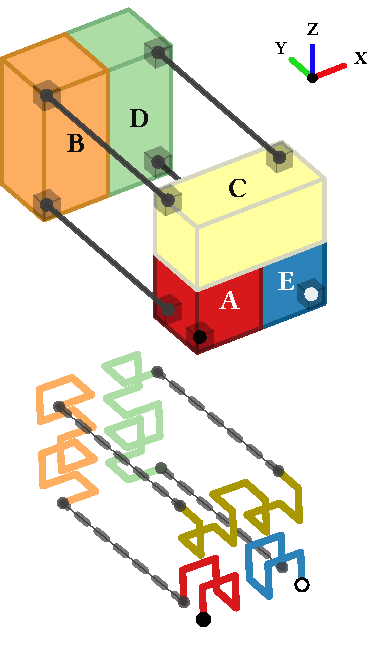
\includegraphics[width=\linewidth]{gilbert3d_explode.pdf}
  \caption{ The $J_0$-split subdivision, representing the main subdivision of the bulk recursion for the 3D Gilbert curve case. }
  \label{fig:gilbert3DJSplit}
\end{figure}

\begin{figure}[h]
  \centering
  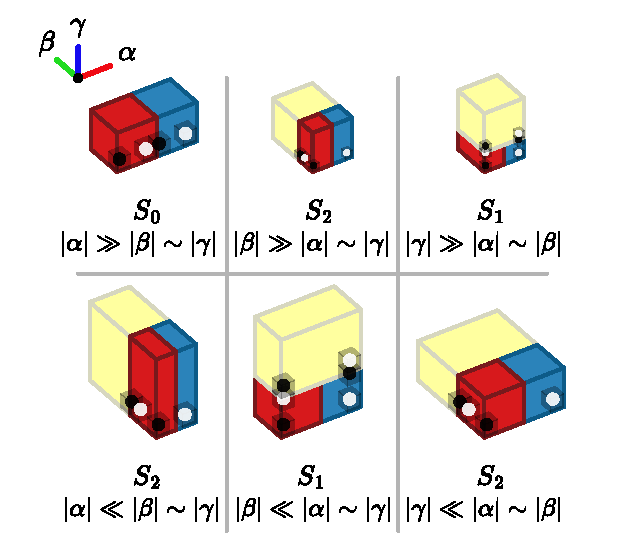
\includegraphics[width=\linewidth]{gilbert3d_eccentric.pdf}
  \caption{ Eccentric cases for recursion. When the cuboid is too far from being cube-like, an $S$-split shape template is used to try and subdivide the cuboids into elements that are more cube like. Here $\alpha$, $\beta$, $\gamma$ are the width-like, height-like and depth-like dimensions. See the text or the algorithm description for the constant ratios used to determine what makes the  cuboid lengths eccentric. }
  \label{fig:gilbert3DEccentricCase}
\end{figure}


The concept of a $U$-split is extended into 3D by constructing a $J$-split.
An exploded view of a $J$-split is shown in Figure \ref{fig:gilbert3DJSplit}.

Side lengths of the subdivided cuboids are chosen to try and not preclude a
Hamiltonian path.
If a path starts at the local $[0,0,0]$, a Hamiltonian path that ends
at $[(w-1),0,0]$ is only possible when $w$ is even or when all lengths are odd, including $w$.


\begin{figure*}[ht]
  \centering
  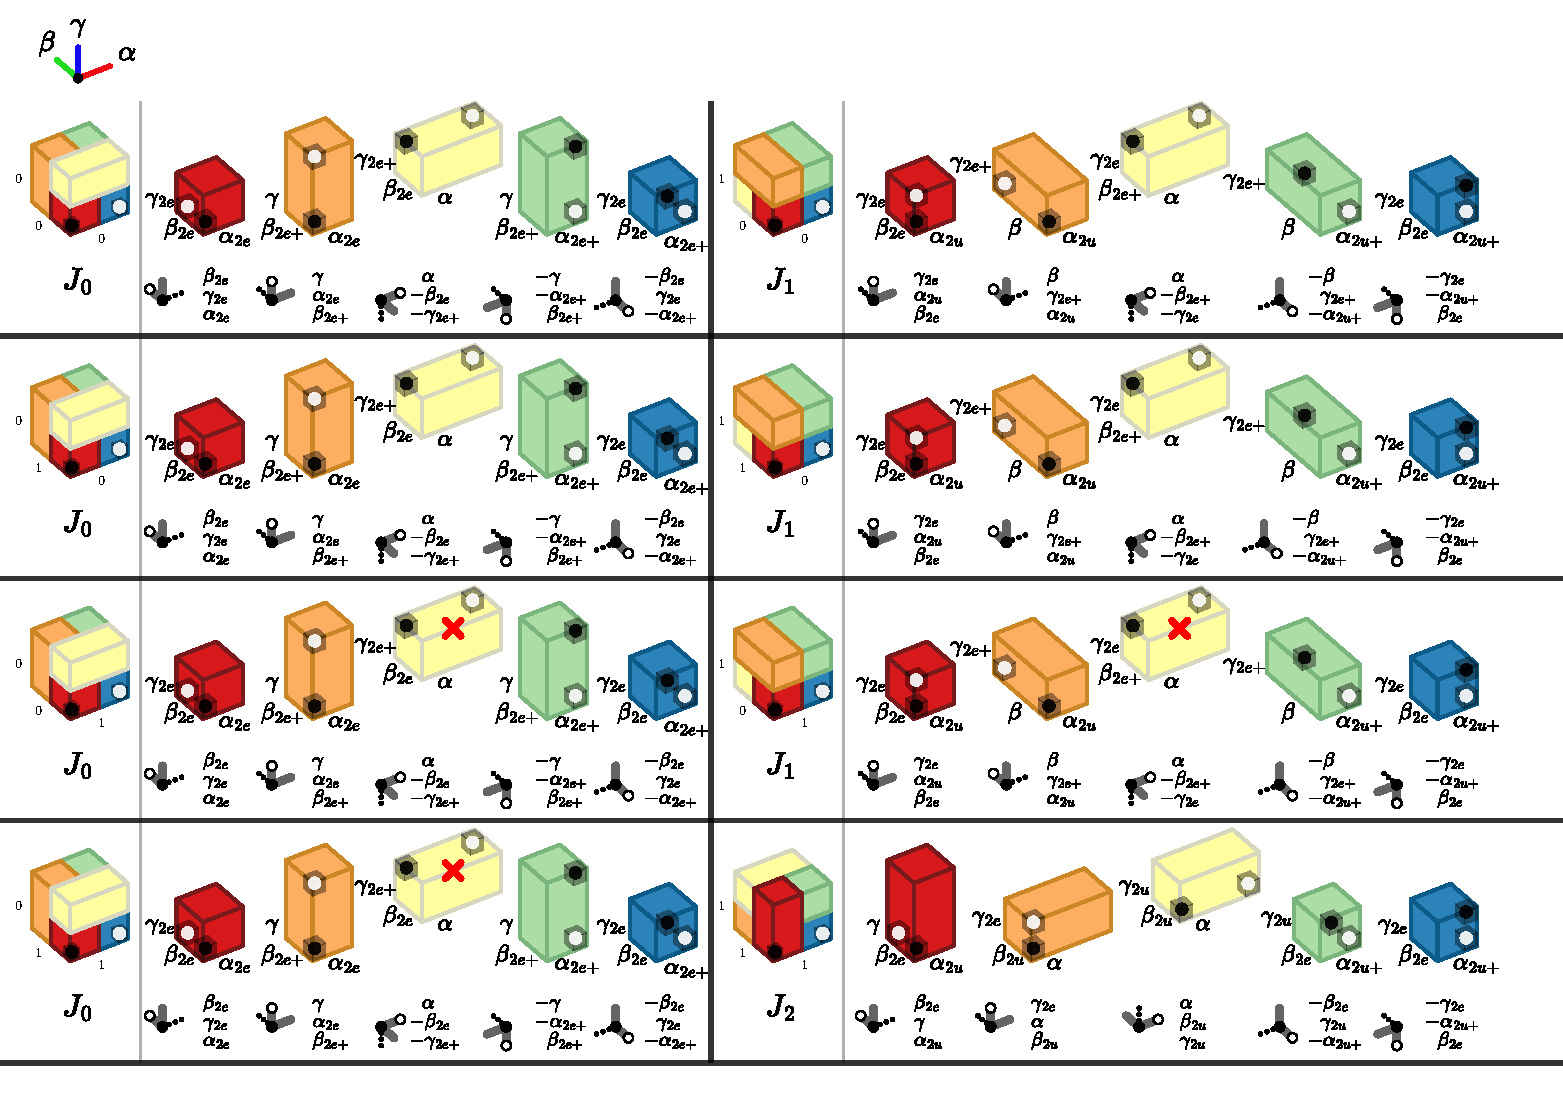
\includegraphics[width=\textwidth]{gilbert3d_case.pdf}
  \caption{ Bulk recursion J-split atlas for the 3D Gilbert algorithm }
  \label{fig:gilbert3DCase}
\end{figure*}

%\floatname{algorithm}{Procedure}
%\begin{algorithm}
%  \caption{ \hskip0.5em $S_0$-Split function (eccentric split) }
%  \label{alg:procS0}
%  \begin{algorithmic}
%    \State
%    \State \textit{\# split halfway on $\alpha$ }
%    \Function{$S_0$}{$p$, $\alpha$, $\beta$, $\gamma$}
%      \State $\alpha_2 \leftarrow (\alpha // 2)$
%      \If{ $(|\alpha| > 2)$ and $((|\alpha_2| \bmod{2}) \equiv 1)$ }
%        \State $\alpha_2 \leftarrow \alpha_2 + \delta(\alpha)$
%      \EndIf
%      \State
%      \State \textbf{yield} Gilbert3D($p$, \\ \hskip8.25em $\alpha_{2}$, $\beta$, $\gamma$ )
%      \State
%      \State \textbf{yield} Gilbert3D($p + \alpha_{2}$, \\ \hskip8.25em $(\alpha - \alpha_{2})$, $\beta$, $\gamma$ )
%    \EndFunction
%  \end{algorithmic}
%\end{algorithm}
%\floatname{algorithm}{Algorithm}
%
%
%\floatname{algorithm}{Procedure}
%\begin{algorithm}
%  \caption{ \hskip0.5em $S_1$-Split functions (eccentric split) }
%  \label{alg:procS1}
%  \begin{algorithmic}
%    \State
%    \State \textit{\# split $\frac{1}{3}$ on $\gamma$ and halfway on $\alpha$ }
%    \Function{$S_1$}{$p$, $\alpha$, $\beta$, $\gamma$}
%      \State $\alpha_2, \gamma_3 \leftarrow (\alpha // 2), (\gamma // 3)$
%      \If{ $(|\alpha| > 2)$ and $((|\alpha_2| \bmod{2}) \equiv 1)$ }
%        \State $\alpha_2 \leftarrow \alpha_2 + \delta(\alpha)$
%      \EndIf
%      \If{ $(|\gamma| > 2)$ and $((|\gamma_3| \bmod{2}) \equiv 1)$ }
%        \State $\gamma_3 \leftarrow \gamma_3 + \delta(\gamma)$
%      \EndIf
%      \State
%      \State \textbf{yield} Gilbert3D($p$, \\ \hskip8.25em $\gamma_3$, $\alpha_2$, $\beta$)
%      \State
%      \State \textbf{yield} Gilbert3D($p + \gamma_3$, \\ \hskip8.25em $\alpha$, $\beta$, $(\gamma - \gamma_3)$)
%      \State
%      \State \textbf{yield} Gilbert3D($p + \alpha - \delta(\alpha) + \gamma_{3} - \delta(\gamma)$, \\ \hskip8.25em $\gamma_3$, $(\alpha - \alpha_2)$, $\beta$)
%    \EndFunction
%  \end{algorithmic}
%\end{algorithm}
%\floatname{algorithm}{Algorithm}
%
%
%\floatname{algorithm}{Procedure}
%\begin{algorithm}
%  \caption{ \hskip0.5em $S_2$-Split function (eccentric split) }
%  \label{alg:procS2}
%  \begin{algorithmic}
%    \State
%    \State \textit{\# split $\frac{1}{3}$ on $\beta$ and halfway on $\alpha$ }
%    \Function{$S_2$}{$p$, $\alpha$, $\beta$, $\gamma$}
%      \State $\alpha_2, \beta_3 \leftarrow (\alpha // 2), (\beta // 3)$
%      \If{ $(|\alpha| > 2)$ and $((|\alpha_2| \bmod{2}) \equiv 1)$ }
%        \State $\alpha_2 \leftarrow \alpha_2 + \delta(\alpha)$
%      \EndIf
%      \If{ $(|\beta| > 2)$ and $((|\beta_3| \bmod{2}) \equiv 1)$ }
%        \State $\beta_3 \leftarrow \beta_3 + \delta(\beta)$
%      \EndIf
%      \State
%      \State \textbf{yield} Gilbert3D($p$, \\ \hskip8.25em $\beta_{3}$, $\gamma$, $\alpha_2$ )
%      \State
%      \State \textbf{yield} Gilbert3D($p + \beta_{3}$, \\ \hskip8.25em $\alpha$, $(\beta - \beta_{3})$, $\gamma$ )
%      \State
%      \State \textbf{yield} Gilbert3D($p + \alpha - \delta(\alpha) + \beta_{3} - \delta(\beta)$, \\ \hskip8.25em $-\beta_{3}$, $\gamma$, $-\alpha$)
%    \EndFunction
%  \end{algorithmic}
%\end{algorithm}
%\floatname{algorithm}{Algorithm}
%
%
%\floatname{algorithm}{Procedure}
%\begin{algorithm}
%  \caption{ \hskip0.5em $J_0$-Split function }
%  \label{alg:procJ0}
%  \begin{algorithmic}
%    \State
%    \State \textit{\# $|\gamma|$ even }
%    \Function{$J_0$}{$p$, $\alpha$, $\beta$, $\gamma$}
%      \State
%      \State $\alpha_2, \beta_2, \gamma_2 \leftarrow (\alpha // 2), (\beta // 2), (\gamma // 2)$
%      \State
%      \State \textit{\# prefer initial block even}
%      \State $\alpha_2=\alpha_2+\delta(\alpha)$ \textbf{if} $(|\alpha_2| > 2)$and$(|\alpha_2| \bmod{2} \equiv 1)$
%      \State $\beta_2=\beta_2+\delta(\beta)$ \textbf{if} $(|\beta_2| > 2)$and$(|\beta_2| \bmod{2} \equiv 1)$
%      \State $\gamma_2=\gamma_2+\delta(\gamma)$ \textbf{if} $(|\gamma_2| > 2)$and$(|\gamma_2| \bmod{2} \equiv 1)$
%      \State
%      \State \textbf{yield} Gilbert3D($p$, \\ \hskip8.25em $\beta_2$, $\gamma_2$, $\alpha_2$)
%      \State
%      \State \textbf{yield} Gilbert3D($p+\beta_2$, \\ \hskip8.25em $\gamma$, $\alpha_2$, $\beta - \beta_2$)
%      \State
%      \State \textbf{yield} Gilbert3D($p + \beta_2 - \delta(\beta_2) + \gamma - \delta(\gamma)$, \\ \hskip8.25em $\alpha$, $-\beta_2$, $-(\gamma - \gamma_2)$)
%      \State
%      \State \textbf{yield} Gilbert3D($p + \alpha - \delta(\alpha) + \beta_2 + \gamma - \delta(\gamma)$, \\ \hskip8.25em $-\gamma$, $-(\alpha - \alpha_2)$, $(\beta - \beta_2)$)
%      \State
%      \State \textbf{yield} Gilbert3D($p + \alpha - \delta(\alpha) + \beta_2 - \delta(\beta)$, \\ \hskip8.25em $-\beta_2$, $\gamma_2$, $-(\alpha - \alpha_2)$)
%    \EndFunction
%  \end{algorithmic}
%\end{algorithm}
%\floatname{algorithm}{Algorithm}


%\floatname{algorithm}{Procedure}
%\begin{algorithm}
%  \caption{ \hskip0.5em $J_1$-Split function }
%  \label{alg:procJ2}
%  \begin{algorithmic}
%    \State
%    \State \textit{\# $|\gamma|$ odd, one of $|\alpha|$ or $|\beta|$ even }
%    \Function{$J_1$}{$p$, $\alpha$, $\beta$, $\gamma$}
%      \State
%      \State $\alpha_2, \beta_2, \gamma_2 \leftarrow (\alpha // 2), (\beta // 2), (\gamma // 2)$
%      \State
%      \State \textit{\# prefer $\beta_2$, $\gamma_2$ even but force $\alpha_2$ odd }
%      \State $\alpha_2=\alpha_2+\delta(\alpha)$ \textbf{if} $(|\alpha_2| > 2)$and$(|\alpha_2| \bmod{2} \equiv 0)$
%      \State $\beta_2=\beta_2+\delta(\beta)$ \textbf{if} $(|\beta_2| > 2)$and$(|\beta_2| \bmod{2} \equiv 1)$
%      \State $\gamma_2=\gamma_2+\delta(\gamma)$ \textbf{if} $(|\gamma_2| > 2)$and$(|\gamma_2| \bmod{2} \equiv 1)$
%      \State
%      \State \textbf{yield} Gilbert3D($p$, \\ \hskip8.25em $\gamma2$, $\alpha_2$, $\beta_2$)
%      \State
%      \State \textbf{yield} Gilbert3D($p+\gamma_2$, \\ \hskip8.25em $\beta$, $\gamma - \gamma_2$, $\alpha_2$)
%      \State
%      \State \textbf{yield} Gilbert3D($p+\gamma_2 - \delta(\gamma) + \beta - \delta(\beta)$, \\ \hskip8.25em $\alpha$, $-(\beta - \beta_2)$, $-\gamma_2$)
%      \State
%      \State \textbf{yield} Gilbert3D($p+\alpha - \delta(\alpha) + \beta - \delta(\beta) + \gamma_2 - \delta(\gamma)$, \\ \hskip8.25em $\beta$, $\gamma - \gamma_2$, $-(\alpha - \alpha_2)$)
%      \State
%      \State \textbf{yield} Gilbert3D($p+\alpha - \delta(\alpha) + \gamma_2 - \delta(\gamma)$, \\ \hskip8.25em $-\gamma_2$, $-(\alpha - \alpha_2)$, $\beta_2$)
%    \EndFunction
%  \end{algorithmic}
%\end{algorithm}
%\floatname{algorithm}{Algorithm}


%\floatname{algorithm}{Procedure}
%\begin{algorithm}
%  \caption{ \hskip0.5em $J_2$-Split function }
%  \label{alg:procJ2}
%  \begin{algorithmic}
%    \State
%    \State \textit{\# $|\alpha|, |\beta|, |\gamma|$ odd }
%    \Function{$J_2$}{$p$, $\alpha$, $\beta$, $\gamma$}
%      \State
%      \State $\alpha_2, \beta_2, \gamma_2 \leftarrow (\alpha // 2), (\beta // 2), (\gamma // 2)$
%      \State
%      \State \textit{\# prefer $\beta_2$, $\gamma_2$ even but force $\alpha_2$ odd }
%      \State $\alpha_2=\alpha_2+\delta(\alpha)$ \textbf{if} $(|\alpha_2| > 2)$and$(|\alpha_2| \bmod{2} \equiv 0)$
%      \State $\beta_2=\beta_2+\delta(\beta)$ \textbf{if} $(|\beta_2| > 2)$and$(|\beta_2| \bmod{2} \equiv 1)$
%      \State $\gamma_2=\gamma_2+\delta(\gamma)$ \textbf{if} $(|\gamma_2| > 2)$and$(|\gamma_2| \bmod{2} \equiv 1)$
%      \State
%      \State \textbf{yield} Gilbert3D($p$, \\ \hskip8.25em $\beta_2$, $\gamma$, $\alpha_2$)
%      \State
%      \State \textbf{yield} Gilbert3D($p+\beta_2$, \\ \hskip8.25em $\gamma_2$, $\alpha$, $(\beta - \beta_2)$)
%      \State
%      \State \textbf{yield} Gilbert3D($p+\beta_2 + \gamma_2$, \\ \hskip8.25em $\alpha$, $(\beta - \beta_2)$, $(\gamma - \gamma_2)$)
%      \State
%      \State \textbf{yield} Gilbert3D($p + \alpha - \delta(\alpha) + \beta_2 - \delta(\beta) + \gamma_2$, \\ \hskip8.25em $-\beta_2$, $(\gamma- \gamma_2)$, $-(\alpha - \delta(\alpha))$)
%      \State
%      \State \textbf{yield} Gilbert3D($p + \alpha - \delta(\alpha) + \gamma_2 - \delta(\gamma)$, \\ \hskip8.25em $-\gamma_2$, $-(\alpha - \alpha_2)$, $\beta_2$)
%    \EndFunction
%  \end{algorithmic}
%\end{algorithm}
%\floatname{algorithm}{Algorithm}


\begin{algorithm}
  \caption{ \hskip0.5em 3D Generalized Hilbert Function (Gilbert3D) } %($p$, $\alpha$, $\beta$, $\gamma$) \\ \hskip3.0em $p, \alpha, \beta, \gamma \in \mathbb{Z}^3$ }
  \label{alg:gilbert3d}
  \begin{algorithmic}
    \State \textit{\# $p, \alpha, \beta, \gamma \in \mathbb{Z}^3$}
    \Function{Gilbert3D}{$p$, $\alpha$, $\beta$, $\gamma$}

    \State
    \State\textit{\# Parity of dimensions}

    \State $\alpha_0 \leftarrow (|\alpha|\bmod{2})$
    \State $\beta_0 \leftarrow (|\beta|\bmod{2})$
    \State $\gamma_0 \leftarrow (|\gamma|\bmod{2})$

    \State
    \State\textit{\# Base cases }
    \State \textbf{if} ($(|\alpha|\equiv 2)$ and $(|\beta|\equiv 2)$ and $(|\gamma| \equiv 2)$)
    \State \hskip1.5em \Return Hilbert3D($p$,$\alpha$,$\beta$,$\gamma$) 
    \State \Return Gilbert2D($p$,$\beta$,$\gamma$) \textbf{if} $(|\alpha| \equiv 1)$
    \State \Return Gilbert2D($p$,$\alpha$,$\gamma$) \textbf{if} $(|\beta| \equiv 1)$
    \State \Return Gilbert2D($p$,$\alpha$,$\beta$) \textbf{if} $(|\gamma| \equiv 1)$

    \State
    \State\textit{\# Eccentric cases }

    \State \textbf{if }$(3 |\alpha|>5|\beta|) \text{ and } (3|\alpha|>5|\gamma|))$
    \State \hskip1.5em \Return $S _ 0$($p$,$\alpha$,$\beta$,$\gamma$) 
    \State \textbf{if }$(2 |\beta| > 3 |\gamma|) \text{ or }(2 |\beta| > 3 |\alpha|))$
    \State \hskip1.5em \Return $S _ 2$($p$,$\alpha$,$\beta$,$\gamma$)
    \State \textbf{if }$(2 |\gamma| > 3 |\beta|)$
    \State \hskip1.5em \Return $S _ 1$($p$,$\alpha$,$\beta$,$\gamma$)

    \State
    \State \textit{\# Bulk recursion }
    \State \Return $J _ 0$($p$,$\alpha$,$\beta$,$\gamma$) \textbf{if} $(\gamma_0 \equiv 0)$
    \State \Return $J _ 1$($p$,$\alpha$,$\beta$,$\gamma$) \textbf{if} $(\alpha_0 \equiv 0)$or$(\beta_0\equiv 0)$
    \State \Return $J _ 2$($p$,$\alpha$,$\beta$,$\gamma$)

    \EndFunction

  \end{algorithmic}
\end{algorithm}



\section{Experiments and Results}

\section{Conclusion}

The Gilbert2D and Gilbert3D provide a generalization of the Hilbert curve to
arbitrary rectangular regions in to two and three dimensions, respectively.
Previous work had side length restrictions, involved complicated algorithms or lacked
easily accessible reference implementations.

Our implementation is conceptually simple, allowing for ease of implementation.
We also provide a libre/free 
reference implementation which can be downloaded from
its repository \footnote{ \label{gilbert-url} \url{https://github.com/jakubcerveny/gilbert}. }

The 2D and 3D Gilbert curve has similar locality metrics to the Hilbert
curve, and provides adequate run-time and memory performance
($O(\lg N)$) for enumeration and random lookup.
When a strict Hamiltonian path is not possible within the desired cuboid volume, the
Gilbert curve provides a ``best-effort'' curve, restricting the inadmissible region
to a single notch point.

Our recursive implementation provides a proof-of-concept for the method.
Further Attempts at memory reductions and constant run-time execution speed optimizations are not pursued in this paper.
There is also a possibility that the shape template subdivision scheme could be extended to higher dimensions but this idea is not
pursued in this paper.







%\bibliographystyle{unsrtnat}
\bibliography{06-References}

\appendix

\clearpage

\section{Appendix}


\subsection{Defect} \label{appendix:defect}

Call the \textit{defect} a function $\lambda _ d : \mathbb{N}^d \mapsto \mathbb{N}$:

$$
\begin{array}{l}
\lambda _ 2 (w,h) = \frac{ w \cdot h }{ \text{min}(w,h)^2 } \\
\lambda _ 3 (w,h,d) = \frac{ w \cdot h \cdot d }{ \text{min}(w,h,d)^3 }
\end{array}
$$

If there is a disjoint subdivision of a volume $V_0$ to $V_1  = ( V _ {0,0}, V _ {0,1}, \dots, V _ {0,m-1} )$,
$V _ 0  = \cup _ {k} V _ {0,k}$,
define the \textit{average defect} of the subdivided volume to be:

$$
\begin{array}{l}
  \lambda _ {s} ( V _ 1 ) = \sum _ {k} \frac{ \text{Vol}(V _ {0,k}) }{ \text{Vol}( V _ 0 ) } \cdot \lambda( V _ {0,k} )
\end{array}
$$

This weights the defect of each subdivided cuboid by its proportional volume.

The defect gives us a coarse idea of how lopsided or \textit{eccentric} a cuboid region is.
If the defect is too high, we might want to split the larger sides while keeping the smaller sides the same size.

\subsection{Eccentric Split Threshold}

Calculations in this section will justify what threshold value to pick of when to choose an
eccentric split over a J-split.
Our concern is to find a simple ratio of when each of $w$, $h$ or $d$ are considered
"small enough" or "large enough", relative to the other dimensions, to split on.

An enumeration of what conditions lead to an eccentric split are as follows:

$$
\begin{array}{ll}
  (1) & w >> h \sim d \\
  (2) & h >> w \sim d \\
  (3) & d >> w \sim h \\
  (4) & h << w \sim d \\
  (5) & w << h \sim d \\
  (6) & d << w \sim h \\
\end{array}
$$

A representation of the eccentric splits are enumerated in Figure \ref{fig:gilbert3DEccentricCase}.
The eccentric $S$-split split differs from the $J$-split as it's only partitioning the cuboid along
one or two dimensions instead of three.

For each of the six cases, we want to know what relative difference in sizes should be used
to determine when an eccentric split should be used and how to subdivide the cuboids so as to make
the resulting subdivided cuboids more cube-like.

Specifically, we want to find the ratio, $\sigma$ or $\eta$, of when one dimension is proportionally larger or smaller,
respectively, than the others.
Further, we choose the ratio, $\rho$, of where to choose the split point of subdivision.
For simplicity, we might want to subdivide at the half way point ($\rho = \frac{1}{2}$) but as we
will see, this might give lopsided sub-cuboid regions and using a better split point is desirable.

In what follows, our goal is to choose a subdivision that will reduce the average defect.
We assume that the start and end of the path lie in the $w$ dimension with the local start point at $(0,0,0)$
and endpoint at $(w-1,0,0)$.

Since the start and end path lie on the $w$ dimension, we are forced to split in the $w$ axis
to subdivide the cuboid.
In what follows, we always commit to splitting the $w$ cuboid region by half, with an
additional coercion step to coerce the $A$ volume to be the desired parity.

\subsection{$|\alpha| >> |\beta| \sim |\gamma|$}

\begin{itemize}
  \item Shape template: $S_0$
  \item $\sigma = \frac{5}{3}$
  \item $\rho = \text{n/a}$
  \item $\eta= \text{n/a}$
\end{itemize}


When $|\alpha|$ is much larger than $|\beta|$ or $|\gamma|$, we only need to split into two sub-cuboids,
which we represent as an $S_0$ split.
As stated above, we pick the midway point for $\alpha$.
What's left is to decide how eccentric the cuboid should be to make the $S_0$ split.

Take $\sigma > 1$:

$$
\begin{array}{l}
  |\alpha| = \sigma s \\
  |\beta| = |\gamma| = s
\end{array}
$$

%Denote the defect of the original volume as $\lambda_0$:
The defect of the original volume is:


$$
\begin{array}{ll}
  \lambda(|\alpha|,|\beta|,|\gamma|)  & = \frac{ |\alpha| \cdot |\beta| \cdot |\gamma| }{ \text{min}(|\alpha|,|\beta|,|\gamma|) } \\
                  & = \frac{ \sigma s \cdot s \cdot s }{ \text{min}(\sigma s,s,s) } \\
                  & = \sigma \\
\end{array}
$$

If $|\alpha| > 2 |\beta| = 2s$, then $\text{min}(\frac{|\alpha|}{2},|\beta|,|\gamma|) = s$ and we have an average defect $\lambda_s(V_1) = \frac{\sigma}{2}$.
Intuitively, we reduce the defect by splitting a long horizontal column into two parts, each of which is more cube like,
making it more cube-like on average.

We can get a better ratio of when to split by asking what the maximum value of $|\alpha| = \sigma s$ is when there is still an average defect reduction.
In this case, we restrict $|\alpha| < 2 |\beta|$, with $\text{min}(\frac{|\alpha|}{2},|\beta|,|\gamma|) = \frac{|\alpha|}{2}$,
the average defect becomes:

$$
\begin{array}{ll}
  \lambda_s(V_1) & = 2 (\frac{1}{2}) \frac{ \frac{\sigma}{2} \cdot s^3 }{ (\frac{\sigma}{2} s)^3 } \\
   & = \frac{4}{\sigma^2}
\end{array}
$$

We want to reduce the average defect relative to the original defect, so:

$$
\begin{array}{ll}
  & \lambda_s (V_1) < \lambda(V_0) \\
  \to & \frac{4}{\sigma^2} < \sigma \\
  \to & 4^{\frac{1}{3}} < \sigma \\ 
  \to & 4^{\frac{1}{3}} = 1.58740\dots < \sigma < \frac{5}{3} \\
\end{array}
$$

For any $\sigma > 4^{\frac{1}{3}}$, we know the average defect will be reduced.
For algorithmic simplicity, we've chosen the simple fraction $\frac{5}{3}$ (as $\frac{5}{3} > 4^{\frac{1}{3}}$)
for the eccentric $S_0$ split ratio.

\subsection{$|\gamma| >> |\alpha| \sim |\beta|$}

\begin{itemize}
  \item Shape template: $S_1$
  \item $\sigma = \frac{3}{2}$
  \item $\rho = \frac{1}{3}$
  \item $\eta= \text{n/a}$
\end{itemize}

Here, we are trying to find two parameters, $\sigma$ as the ratio of when $|\gamma|$ to the minimum
of $|\alpha|$ of $|\beta|$ that indicates we're in an eccentric case, and $\rho$,
the proportion along the $\gamma$ direction of where to choose the split when subdividing the cuboid.

The $S_1$ shape template has three subdivided cuboids, which we call $A$, $B$ and $C$, ordered by
the path traversal through the cuboids.

...





\subsection{$|\beta| >> |\alpha| \sim |\gamma|$}

\begin{itemize}
  \item Shape template: $S_2$
  \item $\sigma = \frac{3}{2}$
  \item $\rho = \frac{3}{2}$
  \item $\eta= \text{n/a}$
\end{itemize}





\clearpage

\section{Auxiliary Algorithms and Procedures} \label{ProcedureAppendix}

\subsection{Auxiliary Functions} \label{AuxiliaryFunctions}

\floatname{algorithm}{Auxiliary Functions}
\begin{algorithm}
  \caption{\hskip0.5em}
  \label{alg:delta}
  \begin{algorithmic}

    \State
    \State \textit{\# integral sign function}
    \Function{$\text{sgn}$}{$w \in \mathbb{Z}$}
      %\State $(w < 0) ? (-1) : ((w > 0) ? 1 : 0)$
      \State \textbf{if} $(w < 0)$ \Return $-1$
      \State \textbf{if} $(w > 0)$ \Return $1$
      \State \Return 0
    \EndFunction

    \State
    \State \textit{\# vector integer round down divide}
    \Function{$\text{div}$}{$v \in \mathbb{Z}^3$, $q \in \mathbb{Z}$ }
      \State $u_0 = \text{sgn}(v_0) \lfloor | \frac{v_0}{q} | \rfloor$
      \State $u_1 = \text{sgn}(v_1) \lfloor | \frac{v_1}{q} | \rfloor$
      \State $u_2 = \text{sgn}(v_2) \lfloor | \frac{v_2}{q} | \rfloor$
      \State \Return $(u_0, u_1, u_2)$
    \EndFunction

    \State
    \State \textit{\# directional vector}
    \Function{$\delta$}{$v \in \mathbb{Z}^3$}
      \State \Return $( \text{sgn}(v_0), \text{sgn}(v_1), \text{sgn}(v_2) )$
    \EndFunction

    \State
    \State \textit{\# Test if $q$ in directional volume with origin $p$}
    \Function{inBounds}{$q, p, \alpha, \beta, \gamma \in \mathbb{Z}^3$}
      \State $v \leftarrow \alpha + \beta + \gamma$
      \For{$i \leftarrow 0$ \textbf{to} $2$}
        \State \textbf{return} \textit{false} \textbf{if} $(\text{sgn}(v_i) \cdot (q_i - p_i) < 0)$
        \State \textbf{return} \textit{false} \textbf{if} $(\text{sgn}(v_i) \cdot (q_i - p_i - v_i) \ge 0)$
      \EndFor
      \State \Return \textit{true}
    \EndFunction

    \State
    \State \textit{\# base case}
    \Function{Hilbert2x2x2}{$p$, $\alpha$, $\beta$, $\gamma$}
      \State \textbf{yield} $p$
      \State \textbf{yield} $p + \delta(\beta)$
      \State \textbf{yield} $p + \delta(\beta) + \delta(\gamma)$
      \State \textbf{yield} $p + \delta(\gamma)$
      \State \textbf{yield} $p + \delta(\alpha) + \delta(\gamma)$
      \State \textbf{yield} $p + \delta(\alpha) + \delta(\beta) + \delta(\gamma)$
      \State \textbf{yield} $p + \delta(\alpha) + \delta(\beta)$
      \State \textbf{yield} $p + \delta(\alpha)$
    \EndFunction

  \end{algorithmic}
\end{algorithm}
\floatname{algorithm}{Algorithm}

\clearpage

\subsection{Gilbert3D S-Split Functions} \label{SSplitFunctions}

\floatname{algorithm}{Procedure}
\begin{algorithm}
  \caption{ \hskip0.5em $S_0$-Split function (eccentric split) }
  \label{alg:procS0}
  \begin{algorithmic}
    \State
    \State \textit{\# split halfway on $\alpha$ }
    \Function{$S_0$}{$p$, $\alpha$, $\beta$, $\gamma$}
      \State $\alpha_2 \leftarrow \text{div}(\alpha, 2)$
      \If{ $(|\alpha| > 2)$ and $((|\alpha_2| \bmod{2}) \equiv 1)$ }
        \State $\alpha_2 \leftarrow \alpha_2 + \delta(\alpha)$
      \EndIf
      \State
      \State \textbf{yield} Gilbert3D($p$, \\ \hskip8.25em $\alpha_{2}$, $\beta$, $\gamma$ )
      \State
      \State \textbf{yield} Gilbert3D($p + \alpha_{2}$, \\ \hskip8.25em $(\alpha - \alpha_{2})$, $\beta$, $\gamma$ )
    \EndFunction
  \end{algorithmic}
\end{algorithm}
\floatname{algorithm}{Algorithm}


\floatname{algorithm}{Procedure}
\begin{algorithm}
  \caption{ \hskip0.5em $S_1$-Split function (eccentric split) }
  \label{alg:procS1}
  \begin{algorithmic}
    \State
    \State \textit{\# split $\frac{1}{3}$ on $\gamma$ and halfway on $\alpha$ }
    \Function{$S_1$}{$p$, $\alpha$, $\beta$, $\gamma$}
      \State $\alpha_2, \gamma_3 \leftarrow \text{div}(\alpha, 2), \text{div}(\gamma, 3)$
      \If{ $(|\alpha| > 2)$ and $((|\alpha_2| \bmod{2}) \equiv 1)$ }
        \State $\alpha_2 \leftarrow \alpha_2 + \delta(\alpha)$
      \EndIf
      \If{ $(|\gamma| > 2)$ and $((|\gamma_3| \bmod{2}) \equiv 1)$ }
        \State $\gamma_3 \leftarrow \gamma_3 + \delta(\gamma)$
      \EndIf
      \State
      \State \textbf{yield} Gilbert3D($p$, \\ \hskip8.25em $\gamma_3$, $\alpha_2$, $\beta$)
      \State
      \State \textbf{yield} Gilbert3D($p + \gamma_3$, \\ \hskip8.25em $\alpha$, $\beta$, $(\gamma - \gamma_3)$)
      \State
      \State \textbf{yield} Gilbert3D($p + \alpha - \delta(\alpha) + \gamma_{3} - \delta(\gamma)$, \\ \hskip8.25em $\gamma_3$, $(\alpha - \alpha_2)$, $\beta$)
    \EndFunction
  \end{algorithmic}
\end{algorithm}
\floatname{algorithm}{Algorithm}


\floatname{algorithm}{Procedure}
\begin{algorithm}
  \caption{ \hskip0.5em $S_2$-Split function (eccentric split) }
  \label{alg:procS2}
  \begin{algorithmic}
    \State
    \State \textit{\# split $\frac{1}{3}$ on $\beta$ and halfway on $\alpha$ }
    \Function{$S_2$}{$p$, $\alpha$, $\beta$, $\gamma$}
      \State $\alpha_2, \beta_3 \leftarrow \text{div}(\alpha, 2), \text{div}(\beta, 3)$
      \If{ $(|\alpha| > 2)$ and $((|\alpha_2| \bmod{2}) \equiv 1)$ }
        \State $\alpha_2 \leftarrow \alpha_2 + \delta(\alpha)$
      \EndIf
      \If{ $(|\beta| > 2)$ and $((|\beta_3| \bmod{2}) \equiv 1)$ }
        \State $\beta_3 \leftarrow \beta_3 + \delta(\beta)$
      \EndIf
      \State
      \State \textbf{yield} Gilbert3D($p$, \\ \hskip8.25em $\beta_{3}$, $\gamma$, $\alpha_2$ )
      \State
      \State \textbf{yield} Gilbert3D($p + \beta_{3}$, \\ \hskip8.25em $\alpha$, $(\beta - \beta_{3})$, $\gamma$ )
      \State
      \State \textbf{yield} Gilbert3D($p + \alpha - \delta(\alpha) + \beta_{3} - \delta(\beta)$, \\ \hskip8.25em $-\beta_{3}$, $\gamma$, $-\alpha$)
    \EndFunction
  \end{algorithmic}
\end{algorithm}
\floatname{algorithm}{Algorithm}

\clearpage

\subsection{Gilbert3D J-Split Functions} \label{JSplitFunctions}

\floatname{algorithm}{Procedure}
\begin{algorithm}
  \caption{ \hskip0.5em $J_0$-Split function }
  \label{alg:procJ0}
  \begin{algorithmic}
    \State
    \State \textit{\# $|\gamma|$ even }
    \Function{$J_0$}{$p$, $\alpha$, $\beta$, $\gamma$}
      \State
      \State $\alpha_2, \beta_2, \gamma_2 \leftarrow \text{div}(\alpha, 2), \text{div}(\beta, 2), \text{div}(\gamma, 2)$
      \State
      \State \textit{\# prefer initial block even}
      \State $\alpha_2 = \alpha_2 + \delta(\alpha)$ \textbf{if} $(| \alpha | > 2)$and$(| \alpha_2 | \bmod{2} \equiv 1)$
      \State $\beta_2 = \beta_2 + \delta(\beta)$ \textbf{if} $(| \beta | > 2)$and$(|\beta_2| \bmod{2} \equiv 1)$
      \State $\gamma_2 = \gamma_2 + \delta(\gamma)$ \textbf{if} $(| \gamma | > 2)$and$(|\gamma_2| \bmod{2} \equiv 1)$
      \State
      \State \textbf{yield} Gilbert3D($p$, \\ \hskip8.25em $\beta_2$, $\gamma_2$, $\alpha_2$)
      \State
      \State \textbf{yield} Gilbert3D($p+\beta_2$, \\ \hskip8.25em $\gamma$, $\alpha_2$, $\beta - \beta_2$)
      \State
      \State \textbf{yield} Gilbert3D($p + \beta_2 - \delta(\beta) + \gamma - \delta(\gamma)$, \\ \hskip8.25em $\alpha$, $-\beta_2$, $-(\gamma - \gamma_2)$)
      \State
      \State \textbf{yield} Gilbert3D($p + \alpha - \delta(\alpha) + \beta_2 + \gamma - \delta(\gamma)$, \\ \hskip8.25em $-\gamma$, $-(\alpha - \alpha_2)$, $(\beta - \beta_2)$)
      \State
      \State \textbf{yield} Gilbert3D($p + \alpha - \delta(\alpha) + \beta_2 - \delta(\beta)$, \\ \hskip8.25em $-\beta_2$, $\gamma_2$, $-(\alpha - \alpha_2)$)
    \EndFunction
  \end{algorithmic}
\end{algorithm}
\floatname{algorithm}{Algorithm}



\floatname{algorithm}{Procedure}
\begin{algorithm}
  \caption{ \hskip0.5em $J_1$-Split function }
  \label{alg:procJ2}
  \begin{algorithmic}
    \State
    \State \textit{\# $|\gamma|$ odd, one of $|\alpha|$ or $|\beta|$ even }
    \Function{$J_1$}{$p$, $\alpha$, $\beta$, $\gamma$}
      \State
      \State $\alpha_2, \beta_2, \gamma_2 \leftarrow \text{div}(\alpha, 2), \text{div}(\beta, 2), \text{div}(\gamma, 2)$
      \State
      \State \textit{\# prefer $\beta_2$, $\gamma_2$ even but force $\alpha_2$ odd }
      \State $\alpha_2=\alpha_2+\delta(\alpha)$ \textbf{if} $(|\alpha| > 2)$and$(|\alpha_2| \bmod{2} \equiv 0)$
      \State $\beta_2=\beta_2+\delta(\beta)$ \textbf{if} $(|\beta| > 2)$and$(|\beta_2| \bmod{2} \equiv 1)$
      \State $\gamma_2=\gamma_2+\delta(\gamma)$ \textbf{if} $(|\gamma| > 2)$and$(|\gamma_2| \bmod{2} \equiv 1)$
      \State
      \State \textbf{yield} Gilbert3D($p$, \\ \hskip8.25em $\gamma_2$, $\alpha_2$, $\beta_2$)
      \State
      \State \textbf{yield} Gilbert3D($p+\gamma_2$, \\ \hskip8.25em $\beta$, $\gamma - \gamma_2$, $\alpha_2$)
      \State
      \State \textbf{yield} Gilbert3D($p+\gamma_2 - \delta(\gamma) + \beta - \delta(\beta)$, \\ \hskip8.25em $\alpha$, $-(\beta - \beta_2)$, $-\gamma_2$)
      \State
      \State \textbf{yield} Gilbert3D($p+\alpha - \delta(\alpha) + \beta - \delta(\beta) + \gamma_2$, \\ \hskip8.25em $\beta$, $\gamma - \gamma_2$, $-(\alpha - \alpha_2)$)
      \State
      \State \textbf{yield} Gilbert3D($p+\alpha - \delta(\alpha) + \gamma_2 - \delta(\gamma)$, \\ \hskip8.25em $-\gamma_2$, $-(\alpha - \alpha_2)$, $\beta_2$)
    \EndFunction
  \end{algorithmic}
\end{algorithm}
\floatname{algorithm}{Algorithm}


\floatname{algorithm}{Procedure}
\begin{algorithm}
  \caption{ \hskip0.5em $J_2$-Split function }
  \label{alg:procJ2}
  \begin{algorithmic}
    \State
    \State \textit{\# $|\alpha|, |\beta|, |\gamma|$ odd }
    \Function{$J_2$}{$p$, $\alpha$, $\beta$, $\gamma$}
      \State
      \State $\alpha_2, \beta_2, \gamma_2 \leftarrow \text{div}(\alpha, 2), \text{div}(\beta, 2), \text{div}(\gamma, 2)$
      \State
      \State \textit{\# prefer $\beta_2$, $\gamma_2$ even but force $\alpha_2$ odd }
      \State $\alpha_2=\alpha_2+\delta(\alpha)$ \textbf{if} $(|\alpha| > 2)$and$(|\alpha_2| \bmod{2} \equiv 0)$
      \State $\beta_2=\beta_2+\delta(\beta)$ \textbf{if} $(|\beta| > 2)$and$(|\beta_2| \bmod{2} \equiv 1)$
      \State $\gamma_2=\gamma_2+\delta(\gamma)$ \textbf{if} $(|\gamma| > 2)$and$(|\gamma_2| \bmod{2} \equiv 1)$
      \State
      \State \textbf{yield} Gilbert3D($p$, \\ \hskip8.25em $\beta_2$, $\gamma$, $\alpha_2$)
      \State
      \State \textbf{yield} Gilbert3D($p+\beta_2$, \\ \hskip8.25em $\gamma_2$, $\alpha$, $(\beta - \beta_2)$)
      \State
      \State \textbf{yield} Gilbert3D($p+\beta_2 + \gamma_2$, \\ \hskip8.25em $\alpha$, $(\beta - \beta_2)$, $(\gamma - \gamma_2)$)
      \State
      \State \textbf{yield} Gilbert3D($p + \alpha - \delta(\alpha) + \beta_2 - \delta(\beta) + \gamma_2$, \\ \hskip8.25em $-\beta_2$, $(\gamma- \gamma_2)$, $-(\alpha - \delta(\alpha))$) 
      \State
      \State \textbf{yield} Gilbert3D($p + \alpha - \delta(\alpha) + \gamma_2 - \delta(\gamma)$, \\ \hskip8.25em $-\gamma_2$, $-(\alpha - \alpha_2)$, $\beta_2$)
    \EndFunction
  \end{algorithmic}
\end{algorithm}
\floatname{algorithm}{Algorithm}


\clearpage

\subsection{Gilbert2D Lookup Functions}

\floatname{algorithm}{Algorithm}
\begin{algorithm}[tbh]
  \caption{\hskip0.5em 2D Generalized Hilbert Index to Position Lookup Function (Gilbert2D\_d2xyz) }
  \label{alg:gilbert2d_d2xyz}
  \begin{algorithmic}

    \State \textit{\# $d_{\text{dst}}, d_{\text{cur}} \in \mathbb{Z}, p, \alpha, \beta \in \mathbb{Z}^3$}
    \Function{Gilbert2D\_d2xyz}{$d_{\text{dst}}$, $d_{\text{cur}}$, $p$, $\alpha$, $\beta$}
      \State
      \State $\alpha_2, \beta_2  = \text{div}(\alpha, 2), \text{div}(\beta, 2)$

      \State
      \If{ $(|\beta| \equiv 1)$ }
        \State \Return $p + (d_{\text{dst}} - d_{\text{cur}}) \cdot \delta(\alpha)$
      \ElsIf{ $(|\alpha| \equiv 1)$ }
        \State \Return $p + (d_{\text{dst}} - d_{\text{cur}}) \cdot \delta(\beta)$

        \State
      \ElsIf{ $(2 |\alpha| > 3 |\beta|)$ }
        \If{ $(|\alpha_2| > 2)$ and $(|\alpha_2| \bmod{2} \equiv 1)$ }
          \State $\alpha_2 \leftarrow \alpha_2 + \delta(\alpha)$
        \EndIf
        \State
        \State $d_{\text{nxt}} \leftarrow d_{\text{cur}} + |\alpha_2| \cdot |\beta|$
        \If{ $d_{\text{cur}} \le d_{\text{dst}} < d_{\text{nxt}}$ }
          \State \Return Gilbert2D\_d2xyz($d_{\text{dst}}$, $d_{\text{cur}}$, \\ \hskip15.0em $p$, \\ \hskip15.0em $\alpha_2$, $\beta$)
        \EndIf
        \State

        \State $d_{\text{cur}} \leftarrow d_{\text{nxt}}$
        \State \Return Gilbert2D\_d2xyz($d_{\text{dst}}$, $d_{\text{cur}}$, \\ \hskip13.5em $p + \alpha_2$, \\ \hskip13.5em $\alpha - \alpha_2$, $\beta$)

        \State
      \EndIf
      \State

      \If{ $(|\beta_2| > 2)$ and $(|\beta_2| \bmod{2} \equiv 1)$ }
        \State $\beta_2 \leftarrow \beta_2 + \delta(\beta)$
      \EndIf
      \State
      \State $d_{\text{nxt}} \leftarrow d_{\text{cur}} + |\beta_2| \cdot |\alpha_2|$
      \If{ $d_{\text{cur}} \le d_{\text{dst}} < d_{\text{nxt}}$ }
        \State \Return Gilbert2D\_d2xyz($d_{\text{dst}}$, $d_{\text{cur}}$, \\ \hskip13.5em $p$, \\ \hskip13.5em $\beta_2$, $\alpha_2$)
      \EndIf
      \State $d_{\text{cur}} \leftarrow d_{\text{nxt}}$
      \State

      \State $d_{\text{nxt}} \leftarrow d_{\text{cur}} + |\alpha| \cdot |\beta-\beta_2|$
      \If{ $d_{\text{cur}} \le d_{\text{dst}} < d_{\text{nxt}}$ }
        \State \Return Gilbert2D\_d2xyz($d_{\text{dst}}$, $d_{\text{cur}}$, \\ \hskip13.5em $p + \beta_2$, \\ \hskip13.5em $\alpha$, $(\beta - \beta_2)$)
      \EndIf
      \State $d_{\text{cur}} \leftarrow d_{\text{nxt}}$
      \State

      \State \Return Gilbert2D\_d2xyz($d_{\text{dst}}$, $d_{\text{cur}}$, \\ \hskip12.0em $p + \alpha - \delta(\alpha) + \beta_2 - \delta(\beta)$, \\ \hskip12.0em $\beta_2$, $-(\alpha - \alpha_2)$)

    \EndFunction
  \end{algorithmic}
\end{algorithm}
\floatname{algorithm}{Algorithm}


\floatname{algorithm}{Algorithm}
\begin{algorithm}[thb]
  \caption{\hskip0.5em 2D Generalized Hilbert Position to Index Lookup Function (Gilbert2D\_xyz2d) }
  \label{alg:gilbert2d_xyz2d}
  \begin{algorithmic}

    \State \textit{\# $d_{\text{cur}} \in \mathbb{Z}, q, p, \alpha, \beta \in \mathbb{Z}^3$}
    \Function{Gilbert2D\_xyz2d}{$d_{\text{cur}}$, $q$, $p$, $\alpha$, $\beta$}
      \State
      \State $\alpha_2, \beta_2  = \text{div}(\alpha, 2), \text{div}(\beta, 2)$

      \State
      \If{ $(|\beta| \equiv 1)$ }
        \State \Return $d_{\text{cur}} + \delta(\alpha) \cdot (q - p)$

        \State
      \ElsIf{ $(|\alpha| \equiv 1)$ }
        \State \Return $d_{\text{cur}} + \delta(\beta) \cdot (q - p)$

        \State
      \ElsIf{ $(2 |\alpha| > 3 |\beta|)$ }
        \If{ $(|\alpha_2| > 2)$ and $(|\alpha_2| \bmod{2} \equiv 1)$ }
          \State $\alpha_2 \leftarrow \alpha_2 + \delta(\alpha)$
        \EndIf
        \State
        \If{ inBounds($q$, $p$, $\alpha_2$, $\beta$) }
          \State \Return Gilbert2D\_xyz2d($p$, \\ \hskip15.0em $\alpha_2$, $\beta$)
        \EndIf
        \State $d_{\text{cur}} \leftarrow d_{\text{cur}} + |\alpha_2| \cdot |\beta|$
        \State

        \State $p \leftarrow p + \alpha_2$
        \State \Return Gilbert2D\_xyz2d($d_{\text{cur}}$, $q$, $p$, \\ \hskip13.5em $\alpha - \alpha_2$, $\beta$)

        \State
      \EndIf

      \If{ $(|\beta_2| > 2)$ and $(|\beta_2| \bmod{2} \equiv 1)$ }
        \State $\beta_2 \leftarrow \beta_2 + \delta(\beta)$
      \EndIf
      \State

      \If{ inBounds($q$, $p$, $\beta_2$, $\alpha_2$) }
        \State \Return  Gilbert2D\_xyz2d($p$, \\ \hskip13.5em $\beta_2$, $\alpha_2$)
      \EndIf
      \State $d_{\text{cur}} \leftarrow d_{\text{cur}} + |\beta_2| \cdot |\alpha_2|$
      \State

      \State $p \leftarrow p + \beta_2$
      \If{ inBounds($q$, $p$, $\alpha$, $(\beta - \beta_2)$) }
        \State \Return Gilbert2D\_xyz2d($d_{\text{cur}}$, $q$, $p$, \\ \hskip13.5em $\alpha$, $(\beta - \beta_2)$)
      \EndIf
      \State $d_{\text{cur}} \leftarrow d_{\text{cur}} + |\alpha| \cdot |\beta - \beta_2|$
      \State

      \State $p \leftarrow p + \alpha - \delta(\alpha) + \beta_2 - \delta(\beta)$
      \State \Return Gilbert2D\_xyz2d($d_{\text{cur}}$, $q$, $p$, \\ \hskip12.0em $\beta_2$, $-(\alpha - \alpha_2)$)

    \EndFunction
  \end{algorithmic}
\end{algorithm}
\floatname{algorithm}{Algorithm}




\end{document}

